%%%%%%%%%%%%%%%%%%%%%%%%%%%%%%%%%%%%%%%%%
% Jacobs Landscape Poster
% LaTeX Template
% Version 1.0 (29/03/13)
%
% Created by:
% Computational Physics and Biophysics Group, Jacobs University
% https://teamwork.jacobs-university.de:8443/confluence/display/CoPandBiG/LaTeX+Poster
% 
% Further modified by:
% Nathaniel Johnston (nathaniel@njohnston.ca)
%
% This template has been downloaded from:
% http://www.LaTeXTemplates.com
%
% 
% Masaryk University presentation themes were downloaded from:
% https://www.overleaf.com/gallery/tagged/muni
%
% and ported into Jacobs Landscape Poster by:
% Jumaidil Awal (ideal1st.here@googlemail.com)
% 
% Jacobs Landscape Poster License:
% CC BY-NC-SA 3.0 (http://creativecommons.org/licenses/by-nc-sa/3.0/)
%
% Masaryk University's fibeamer theme license:
% Copyright 2015  Vít Novotný <witiko@mail.muni.cz>
% Faculty of Informatics, Masaryk University (Brno, Czech Republic)
% under Latex Project Public License
%
%%%%%%%%%%%%%%%%%%%%%%%%%%%%%%%%%%%%%%%%%

%----------------------------------------------------------------------------------------
%	PACKAGES AND OTHER DOCUMENT CONFIGURATIONS
%----------------------------------------------------------------------------------------

\documentclass[final]{beamer}

\usepackage[scale=1.24]{beamerposter} % Use the beamerposter package for laying out the poster

%\usetheme{confposter} % Use the confposter theme supplied with this template
\usetheme[faculty=chemo]{fibeamer} % Uncomment to use Masaryk University's fibeamer theme instead.

%\setbeamercolor{block title}{fg=ngreen,bg=white} % Colors of the block titles
%\setbeamercolor{block body}{fg=black,bg=white} % Colors of the body of blocks
%\setbeamercolor{block alerted title}{fg=white,bg=dblue!70} % Colors of the highlighted block titles
%\setbeamercolor{block alerted body}{fg=black,bg=dblue!10} % Colors of the body of highlighted blocks
% Many more colors are available for use in beamerthemeconfposter.sty

%-----------------------------------------------------------
% Define the column widths and overall poster size
% To set effective sepwid, onecolwid and twocolwid values, first choose how many columns you want and how much separation you want between columns
% In this template, the separation width chosen is 0.024 of the paper width and a 4-column layout
% onecolwid should therefore be (1-(# of columns+1)*sepwid)/# of columns e.g. (1-(4+1)*0.024)/4 = 0.22
% Set twocolwid to be (2*onecolwid)+sepwid = 0.464
% Set threecolwid to be (3*onecolwid)+2*sepwid = 0.708

\newlength{\sepwid}
\newlength{\onecolwid}
\newlength{\twocolwid}
\newlength{\threecolwid}
\setlength{\paperwidth}{46.8in} % A0 width: 46.8in
\setlength{\paperheight}{33.1in} % A0 height: 33.1in
\setlength{\sepwid}{0.024\paperwidth} % Separation width (white space) between columns
\setlength{\onecolwid}{0.21\paperwidth} % Width of one column
\setlength{\twocolwid}{0.451\paperwidth} % Width of two columns
\setlength{\threecolwid}{0.678\paperwidth} % Width of three columns
%\setlength{\topmargin}{-0.5in} % Reduce the top margin size
%-----------------------------------------------------------

\usepackage{graphicx}  % Required for including images

\usepackage{booktabs} % Top and bottom rules for tables

%----------------------------------------------------------------------------------------
%	TITLE SECTION 
%----------------------------------------------------------------------------------------

\title{Function 7 : $a^{b^x}$} % Poster title

\author{Deliverable 4} % Author(s)

\institute{SOEN-6011 Software Engineering Processes} % Institution(s)

%----------------------------------------------------------------------------------------

\begin{document}
\addtobeamertemplate{block end}{}{\vspace*{2ex}} % White space under blocks
\addtobeamertemplate{block example end}{}{\vspace*{2ex}} % White space under example blocks
\addtobeamertemplate{block alerted end}{}{\vspace*{2ex}} % White space under highlighted (alert) blocks

\setlength{\belowcaptionskip}{2ex} % White space under figures
\setlength\belowdisplayshortskip{2ex} % White space under equations
%\begin{darkframes} % Uncomment for dark theme, don't forget to \end{darkframes}
\begin{frame} % The whole poster is enclosed in one beamer frame

%==========================Begin Head===============================

  \begin{columns}
   \begin{column}{\linewidth}
    \vskip1cm
    \centering
    \usebeamercolor{title in headline}{\color{fg}\Huge{\textbf{\inserttitle}}\\[0.5ex]}
    \usebeamercolor{author in headline}{\color{fg}\Large{\insertauthor}\\[1ex]}
    \usebeamercolor{institute in headline}{\color{fg}\large{\insertinstitute}\\[1ex]}
    \vskip1cm
   \end{column}
   \vspace{1cm}
  \end{columns}
 \vspace{1cm}

%==========================End Head===============================

\begin{columns}[t] % The whole poster consists of three major columns, the second of which is split into two columns twice - the [t] option aligns each column's content to the top

\begin{column}{\sepwid}\end{column} % Empty spacer column

\begin{column}{\onecolwid} % The first column

%----------------------------------------------------------------------------------------
%	OBJECTIVES
%----------------------------------------------------------------------------------------

\begin{exampleblock}{Desideratum implementation}
The current version has the following implementation : \\ 
\begin{itemize}

\item Memento of the user interactions using Memento design pattern
\item Displaying accurate user results
\item Performing accurate results without by the core implementation of the transcendental function
\item The calculation of Taylor series and logarithmic function
\item Using User interface patterns to improve usability
\item Supports both the GUI and command interface by changing execution 
\item Making a correct, efficient, maintainable, robust and usable system
\item Maintaining an accuracy and precision with a normal calculator
\item Handling both the cases of the integers and decimal powers to provide
precise results
\item Verifying inputs and outputs as real numbers.
\item Proper domain verification

\end{itemize}

\end{exampleblock}

%----------------------------------------------------------------------------------------
%	INTRODUCTION
%----------------------------------------------------------------------------------------

\begin{exampleblock}{Current Version}
\begin{itemize}
    \item All tasks achieved 
    \item Good reviews reported by fellow team mates
    \item Interactive GUI improved user experience
    \item Memento pattern help achieve user history
\end{itemize}
\end{exampleblock}


\end{column} % End of the first column

\begin{column}{\sepwid}\end{column} % Empty spacer column

\begin{column}{\twocolwid} % Begin a column which is two columns wide (column 2)

\begin{columns}[t,totalwidth=\twocolwid] % Split up the two columns wide column

\begin{column}{\onecolwid}\vspace{-.74in} % The first column within column 2 (column 2.1)

%----------------------------------------------------------------------------------------
%	MATERIALS
%----------------------------------------------------------------------------------------

\begin{exampleblock}{Critical Decisions [Formulas]}

\begin{itemize}
    \item 1. Decision: The implementation of the Taylor series helped with the precision of up-to 50 points of the decimal places by morphing the function $a^{b^x}$ to two parts, specifically y = $e^{x * \log{b}}$ and z = $\exp^{y * \log{a}}$, where 'z' is the final result of the expression. \\
    Result: The implementation of the Taylor series helped achieved accurate results.
\item Decision: The calculation of the log function with the base 10 instead of the natural log and converting the result. \\
Result: The implementation of the $log_{10}$ was much easier and with the simple formula \\ $\log_e (x) = \frac{\log_{10} (x)}{\log_{10} (e)}$

\end{itemize}
\end{exampleblock}
\begin{exampleblock}{Critical Decisions [Coding]}
\begin{itemize}
    \item \textbf{GUI interface:} Code contains implementation of both command line and graphical interface. But ease of use GUI was preferred.  
    \item \textbf{Memento Pattern:} The memorization of last calculation for the user's convenience aimed to make real world calculator. 
\end{itemize}
\end{exampleblock}
%----------------------------------------------------------------------------------------

\end{column} % End of column 2.1
\begin{column}{\sepwid}\end{column} % Empty spacer column

\begin{column}{\onecolwid}\vspace{-.74in} % The second column within column 2 (column 2.2)

%----------------------------------------------------------------------------------------
%	METHODS
%----------------------------------------------------------------------------------------

\begin{exampleblock}{Critical Decision}

\begin{enumerate}
\item \textbf{Dual Implementation: } The results with normal Taylor series and logarithmic function provided irregular results with integer power. To get specific result the integer version of the code was implemented.
\item \textbf{Testing: } The aim of the calculator was to provide accurate results but every calculator is implemented in different ways. So for proper testing the decimal precision was set up to 5 and 4 in some cases.
\item \textbf{Exception Handling: } The decision was to print the exception messages as coder also so implementer can understand the specific working. Or to be user specific. The proper usage of 'JOptionPane' represented the message in the UI based interface.
\item \textbf{Rounding Digits: } Rounding digits for normal numbers had no problems but with large numbers the exponent value got dropped off. So, the decision was made to remove the rounding off numbers.
\item \textbf{Messaging: }Proper messages and information of the function was specified in the interface.
\end{enumerate}
\end{exampleblock}

%----------------------------------------------------------------------------------------

\end{column} % End of column 2.2

\end{columns} % End of the split of column 2 - any content after this will now take up 2 columns width

%----------------------------------------------------------------------------------------
%	GUI Representation
%----------------------------------------------------------------------------------------

\begin{alertblock}{\centering Graphical Interface}
\begin{figure}
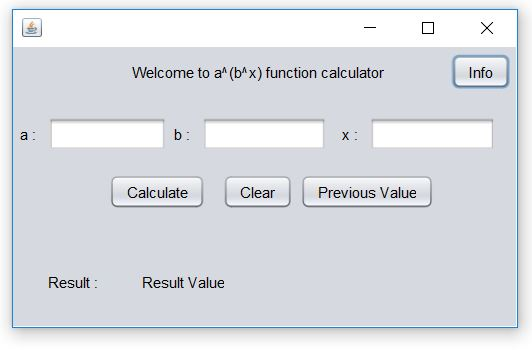
\includegraphics[height= 0.35 \linewidth]{Calculator_image.JPG}
\end{figure}
\end{alertblock} 

%----------------------------------------------------------------------------------------

\begin{columns}[t,totalwidth=\twocolwid] % Split up the two columns wide column again

\begin{column}{\onecolwid} % The first column within column 2 (column 2.1)

%----------------------------------------------------------------------------------------
%	MATHEMATICAL SECTION
%----------------------------------------------------------------------------------------



%----------------------------------------------------------------------------------------

\end{column} % End of column 2.1
\begin{column}{\sepwid}\end{column} % Empty spacer column

\begin{column}{\onecolwid} % The second column within column 2 (column 2.2)

%----------------------------------------------------------------------------------------
%	RESULTS
%----------------------------------------------------------------------------------------


%----------------------------------------------------------------------------------------

\end{column} % End of column 2.2

\end{columns} % End of the split of column 2

\end{column} % End of the second column

\begin{column}{\sepwid}\end{column} % Empty spacer column

\begin{column}{\onecolwid} % The third column

%----------------------------------------------------------------------------------------
%	Improvements
%----------------------------------------------------------------------------------------

\begin{exampleblock}{Improvements}
\begin{itemize}
    \item Rounding off Results : One of the future improvements were the rounding off the results.
    \item Memento: Improving the memento pattern to store the results of last 10 calculations and adding buttons to use value in new calculations.
    \item Interface : The code consists proper working for GUI and command line. An addendum would be to giver user the choice of working with the interface user wants.
    \item Exponent Dropping: New improvement for the code was to round off numbers without using internal libraries and find a way to manage the exponent
    \item Bounding Improvement: The biggest value in Java is double's max value, but improving max boundary further to have precise results. 
\end{itemize}
\end{exampleblock}

%----------------------------------------------------------------------------------------
%	ADDITIONAL INFORMATION
%----------------------------------------------------------------------------------------

\begin{exampleblock}{Lessons Learned}
\begin{itemize}
\item Implementation and learning of Memento Design Pattern
\item Improving testing and java docs 
\item Core function implementation of Log function and Taylor Series
\item Proper IEEE documentation methods
\item Managing workings with team members.
\end{itemize}

\end{exampleblock}



%----------------------------------------------------------------------------------------
%	CONTACT INFORMATION
%----------------------------------------------------------------------------------------

%\setbeamercolor{block alerted title}{fg=black,bg=norange} % Change the alert block title colors
%\setbeamercolor{block alerted body}{fg=black,bg=white} % Change the alert block body colors

\begin{block}{Contact Information}

\begin{itemize}
\item Himanshu Kohli [ID: 40070839, Team-E]
\item GitHub: \url{https://github.com/Hkohli30/SOEN_6011}
\end{itemize}

\end{block}

\end{column} % End of the third column

\begin{column}{\sepwid}\end{column} % Empty spacer column

\end{columns} % End of all the columns in the poster

\end{frame} % End of the enclosing frame
%\end{darkframes} % Uncomment for dark theme
\end{document}
